\documentclass{beamer}

\usepackage[francais]{babel}
\usepackage[utf8]{inputenc}
\usepackage[T1]{fontenc}
\usepackage{graphicx}
\usepackage{graphics}
\usepackage{color}
\usepackage{textcomp}
\usepackage{pifont}
\usepackage[normalem]{ulem}
\usepackage{times}
\usepackage{hyperref}
\usepackage{verbatim}
\usepackage{amsmath}
\usepackage{amsthm}
\usepackage{amsfonts}
\usepackage[mathscr]{euscript}
\usepackage{pgfpages}
\usepackage{listings}
\usepackage{subfigure}
\usepackage{algorithm}
\usepackage[noend]{algorithmic}
\usepackage{pdftricks}
\usepackage{mathrsfs}
\usepackage{array}
\usepackage{fancybox}
% \usepackage{columns}
\usepackage{multirow}
\usepackage{url}
\usepackage{tikz}
\usepackage{colortbl}
%\usepackage{cite} %DO NOT FUCKING USE CITE ON BEAMER !!! LOST 30 GODDAM' MINUTES ON THIS SHIT !!!
\usepackage{mathabx}
\usepackage{amssymb}
\usepackage{eurosym}
\usepackage{wasysym} % ch0

\let\texteuro\euro

\hypersetup{colorlinks,%
            citecolor=black,%
            filecolor=black,%
            linkcolor=black,%
            urlcolor=blue}

%\addtolength{\parskip}{10pt}

\usetikzlibrary{calc}

\mode<presentation>
\setbeamertemplate{footline}[frame number]
\setbeamercovered{transparent}
\usetheme[navigation]{ESI}

%lst
\definecolor{comment-green}{RGB}{0,166,80}
\lstset{language=C++,
  keywordstyle=\lst@ifdisplaystyle\bf\fi\color{blue!60},
  commentstyle=\color{comment-green},
  stringstyle=\color{red},
  basicstyle=\lst@ifdisplaystyle\tiny\else\tt\fi,
  morekeywords={
    constexpr,concept,decltype,nullptr,nullptr_t,noexcept,final,override},
  frame=single,
  xleftmargin=0.5cm,
  numbers=left,
  tabsize=2}

%title
\subtitle{Langage \texttt{C} / \cpp}
\author{R. Absil}
\date{\today}

%styles
\theoremstyle{definition}
\newtheorem{thm}{Théorème}
\newtheorem{conj}[thm]{Conjecture}
\newtheorem{deff}[thm]{Définition}
\newtheorem{prop}[thm]{Propriété}
\newtheorem{lem}[thm]{Lemme}
\newtheorem*{lem*}{Lemme}
\newtheorem{cor}[thm]{Corollaire}
%\newtheorem{example}{Exemple}
\newtheorem{remark}{Remarque}
\newtheorem{exo}{Exercice}

%typeset
\newcommand{\ie}{{\emph{i.e., }}}
\newcommand{\eg}{{\emph{e.g., }}}
\newcommand{\etal}{{\emph{et al.}}}
\newcommand{\rrceil}{\unichar{"2308}}
\newcommand{\sloand}[2]{\footnote{N. J. A. Sloane - OEIS Foundation - \texttt{www.oeis.org}, Sequence #1 - #2.}}

%math
\newcommand{\IN}{{\mathbb N}}
\newcommand{\IQ}{{\mathbb Q}}
\newcommand{\IR}{{\mathbb R}}
\newcommand{\IZ}{{\mathbb Z}}
\newcommand{\IP}{{\mathbb P}}
\newcommand{\IC}{{\mathbb C}}
\newcommand{\bigo}{{\mathcal{O}}}
\renewcommand{\mod}{\bmod}
\newcommand{\ssi}{\Leftrightarrow}
\newcommand{\then}{\Rightarrow}
\newcommand{\fle}[1]{\stackrel{#1}{\longrightarrow}}
\newcommand{\suchthat}{~\big|~}
\newcommand{\floor}[1]{\left\lfloor #1 \right\rfloor}
\newcommand{\ceil}[1]{\left\lceil #1 \right\rceil}
\DeclareMathOperator*{\argmin}{argmin}
\DeclareMathOperator*{\argmax}{argmax}

%tikz
\tikzstyle{_vertex}=[fill=white, circle,minimum size=12pt,inner sep=1pt]
\tikzstyle{_blackv}=[fill=black, circle,minimum size=8pt,inner sep=1pt]
\tikzstyle{_dot}=[fill=black, circle, minimum size = 1mm, inner sep=0pt]
\tikzstyle{_bigvertex}=[fill=white, circle,minimum size=21pt,inner sep=1pt]
\tikzstyle{_arc}=[->, >=stealth]
\tikzstyle{_boldarc}=[->, >=stealth, line width=2pt]

\newcommand{\cpp}{\texttt{C++}}
\newcommand{\java}{\texttt{Java}}


\title{Ch. 3 - Fonctions}

\begin{document}
\begin{frame}
  \titlepage
\end{frame}

\begin{frame}
  \frametitle{Table des matières}
  \footnotesize \tableofcontents[pausesections,pausesubsections]
\end{frame}


\section{Introduction}

\begin{frame}
\frametitle{Utilité}
\begin{itemize}[<+->]
\item «~Ensemble d'instructions qui effectue une tâche~»
\item Peut être \emph{appelé} au sein d'un programme
\end{itemize}
\begin{exampleblock}<+->{Avantages}
	\begin{itemize}[<+->]
	\item Permet de découper le travail en parties indépendantes
	\item Permet de réutiliser du code
	\item Limite la redondance
		\begin{itemize}
		\item Moins de « copier / coller »
		\item Maintenabilité augmentée
		\end{itemize}
	\item Augmente la lisibilité
	\end{itemize}
\end{exampleblock}
\end{frame}

\begin{frame}
\frametitle{Caractéristiques}
\begin{enumerate}[<+->]
\item Possède des paramètres et un retour
	\begin{itemize}
	\item \texttt{sqrt} prend en paramètre un flottant et retourne un flottant
	\end{itemize}
\item Identifiées par leur nom et leurs paramètres
	\begin{itemize}
	\item Les règles d'appel sont appliquées sur ces caractéristiques
	\item \emph{Pas} le type de retour
	\end{itemize}
\item Concept indépendant de la POO
	\begin{itemize}
	\item Fonctions \emph{membres} (méthodes : \cpp)
	\item Fonctions indépendantes
	\end{itemize}
\item Plus qu'une fonction mathématique
	\begin{itemize}
	\item Effectue un travail
	\item Possibilité de modifier les paramètres
	\item Peut ne rien retourner (\lstinline|void|)
	\end{itemize}
\end{enumerate}
\end{frame}

\begin{frame}
\frametitle{Déclaration et définition}
\begin{itemize}
\onslide<1-> \item Toute fonction doit être déclarée et définie
	\begin{itemize}
	\onslide<2->\item Possibilité de séparer la déclaration de la définition
	\onslide<3->\item Parfois nécessaire
	\end{itemize}
\end{itemize}
\begin{center}
\visible<4-|handout:1>{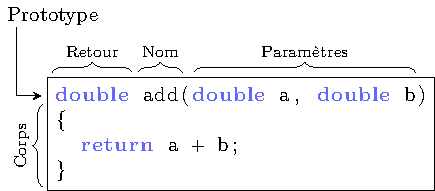
\includegraphics[width=.7\textwidth]{pics/fct.pdf}}
\end{center}
\begin{itemize}
\onslide<5-> \item Seul les types des paramètres sont nécessaires dans le prototype
\onslide<6-> \item Les fonctions \emph{doivent} être déclarées avant d'être utilisées
\onslide<7-> \item Déclaration possible au sein d'un bloc
\end{itemize}
\end{frame}

\begin{frame}[containsverbatim]
\frametitle{Exemple}
\begin{itemize}
\item Fichier \texttt{before.c}
\end{itemize}
\begin{lstlisting}
int main()
{
	print("Hello");
}

void print(const char* s)
{
	printf("%s\n", s);
}
\end{lstlisting}
\begin{itemize}
\item Déclaration anticipée
\end{itemize}
\begin{lstlisting}
void print(const char*);

int main()
{
	print("Hello");
}

void print(const char* s)
{
	printf("%s\n", s);
}
\end{lstlisting}
\begin{itemize}
\item Même principe en \cpp
\end{itemize}
\end{frame}

\begin{frame}[containsverbatim]
\frametitle{Les fonctions sans arguments en \texttt{C}}
\begin{itemize}
\item En \texttt{C} uniquement, si on veut qu'une fonction n'accepte aucun argument, il faut écrire \lstinline|void| dans la liste des paramètres
\item Si on déclare \lstinline|void f();|, la fonction \texttt{f} accepte un nombre arbitraire d'arguments (et les ignore)
\end{itemize}
\begin{lstlisting}
void f() {}
void g(void) {}

int main()
{
    f();
    f(1); //ok
    f(1,2); //ok
    
    g();
    //g(1); //ko    
}
\end{lstlisting}
\end{frame}

\section{Passage d'argument}

\begin{frame}
\frametitle{Passage par valeur}
\begin{itemize}[<+->]
\item Par défaut, à chaque appel d'une fonction, une \emph{copie} des paramètres est envoyée à la fonction
	\begin{itemize}
	\item Dans le cas d'un type de base, on copie la valeur
	\item Dans le cas d'une \lstinline|struct| (\texttt{C}), on copie les attributs
	\item Dans le cas d'un objet (\cpp), on appelle le constructeur de recopie (cf. Ch. 4)
	\end{itemize}
\item « Ne permet pas » de modifier les paramètres
\item La valeur de retour est également transmise par valeur	
\end{itemize}
\begin{exampleblock}<+->{Avantages}
	\begin{itemize}[<+->]
	\item Pas d'effet de bord
	\end{itemize}
\end{exampleblock}
\begin{alertblock}<+->{Inconvénients}
	\begin{itemize}[<+->]
	\item Performances réduites
	\end{itemize}
\end{alertblock}
\end{frame}

\begin{frame}
\frametitle{Mécanisme}
\begin{center}
\begin{tikzpicture}
\node[draw] at (0,0) 
{
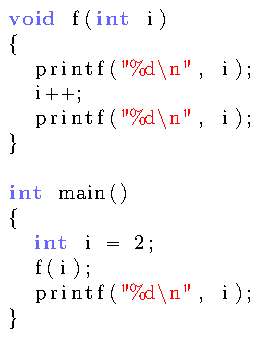
\includegraphics[width=4cm]{pics/sample-value.pdf}
};

\node at (7.5,3.5) {Pile};
\draw (6,-3) -- (6,3);
\draw (9,-3) -- (9,3);

%\foreach \i in {-2.5,-2,...,2.5}
%	\draw (6,\i) -- (9,\i);
\draw (6,-2.75) -- (9,-2.75);
\draw (6,2.75) -- (9,2.75);

\only<1->{\draw[white,->,>=stealth,ultra thick] (-2.8,-0.75) -- (-2.3,-0.75);} %phantom
\only<2>{\draw[comment-green,->,>=stealth,ultra thick] (-2.8,-0.75) -- (-2.3,-0.75);}
\only<3>{\draw[comment-green,->,>=stealth,ultra thick] (-2.8,-1.1) -- (-2.3,-1.1);}
\only<4>{\draw[comment-green,->,>=stealth,ultra thick] (-2.8,-1.5) -- (-2.3,-1.5);}
\only<5>{\draw[comment-green,->,>=stealth,ultra thick] (-2.8,2.25) -- (-2.3,2.25);}
\only<6>{\draw[comment-green,->,>=stealth,ultra thick] (-2.8,1.5) -- (-2.3,1.5);}
\only<7>{\draw[comment-green,->,>=stealth,ultra thick] (-2.8,1.1) -- (-2.3,1.1);}
\only<8>{\draw[comment-green,->,>=stealth,ultra thick] (-2.8,0.75) -- (-2.3,0.75);}
\only<9>{\draw[comment-green,->,>=stealth,ultra thick] (-2.8,0.4) -- (-2.3,0.4);}
\only<10>{\draw[comment-green,->,>=stealth,ultra thick] (-2.8,-1.9) -- (-2.3,-1.9);}

%\only<3->{\node at (5.25,-2.35) {\scriptsize \texttt{0xCAFE}};}
\only<3->{\filldraw[blue!60, fill=blue!60, rounded corners=2mm] (6.1,-2.65) rectangle (8.9,-2.05) node[midway,black] {$2$};}
\only<3->{\node at (5.75,-2.35) {\scriptsize \texttt{i}};}

\only<5-6>{\filldraw[blue!60, fill=blue!60, rounded corners=2mm] (6.1,1) rectangle (8.9,1.6) node[midway,black] {$2$};}
\only<7-8>{\filldraw[blue!60, fill=blue!60, rounded corners=2mm] (6.1,1) rectangle (8.9,1.6) node[midway,black] {$3$};}
\only<5-8>{\node at (5.1,1.3) {\scriptsize Copie de \texttt{i}};}

\only<9->{\filldraw[blue!10, fill=blue!10, rounded corners=2mm] (6.1,1) rectangle (8.9,1.6) node[midway,black!30] {$3$};}
\only<9->{\node[black!30] at (5.1,1.3) {\scriptsize Copie de \texttt{i}};}
\end{tikzpicture}
\end{center}
\end{frame}

\begin{frame}[containsverbatim]
\frametitle{Mauvais swap}
\begin{itemize}
\item Fichier \texttt{swap-value.cpp}
\end{itemize}
\begin{lstlisting}
void swap(int x, int y)
{
	cout << "Entering swap : " << x << " " << y << endl;	

	int tmp = y;
	y = x;
	x = tmp;

	cout << "Exiting swap : " << x << " " << y << endl;
}

int main()
{
	int i = 1;
	int j = 2;

	cout << "Before call : " << i << " " << j << endl;
	swap(i, j);
	cout << "After call : " << i << " " << j << endl;
}
\end{lstlisting}
\end{frame}

\begin{frame}[containsverbatim]
\frametitle{Exemple}
\begin{itemize}
\item Fichier \texttt{pass-value.cpp}
\end{itemize}
\begin{lstlisting}
void countDown(int i)
{
	while(i > 0)
	{
		cout << i << endl;
		i--;
	}
	cout << "BOOM" << endl;
}

int main()
{
	for(int i = 5; i >= 0; i--)
	{
		countDown(i);
		cout << endl;
	}
}
\end{lstlisting}
\end{frame}

\begin{frame}
\frametitle{Passage par adresse}
\begin{itemize}[<+->]
\item On ne transmet pas une copie de l'objet, mais son adresse
	\begin{itemize}
	\item « Comme en \java\ »
	\end{itemize}
\item Permet d'émuler un passage par référence
	\begin{itemize}
	\item En \texttt{C} pur, pas d'autre solution
	\end{itemize}
\end{itemize}
\begin{alertblock}<+->{Inconvénients par rapport aux références}
	\begin{itemize}[<+->]
	\item Plus «~risqué~»
		\begin{itemize}
		\item Hygiène de programmation plus stricte
		\end{itemize}
	\item Syntaxe «~moins transparente~»
	\end{itemize}
\end{alertblock}
\begin{itemize}[<+->]
\item Parfois (rarement) pas d'autre choix en \cpp
\end{itemize}
\end{frame}

\begin{frame}
\frametitle{Mécanisme}
\begin{center}
\begin{tikzpicture}
\node[draw] at (0,0) 
{
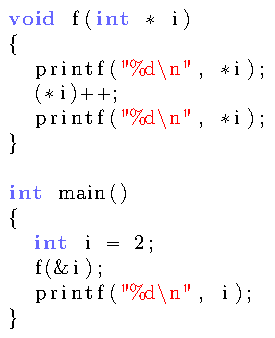
\includegraphics[width=4cm]{pics/sample-address.pdf}
};

\node at (7.5,3.5) {Pile};
\draw (6,-3) -- (6,3);
\draw (9,-3) -- (9,3);

%\foreach \i in {-2.5,-2,...,2.5}
%	\draw (6,\i) -- (9,\i);
\draw (6,-2.75) -- (9,-2.75);
\draw (6,2.75) -- (9,2.75);

\only<1->{\draw[white,->,>=stealth,ultra thick] (-2.8,-0.75) -- (-2.3,-0.75);} %phantom
\only<2>{\draw[comment-green,->,>=stealth,ultra thick] (-2.8,-0.75) -- (-2.3,-0.75);}
\only<3>{\draw[comment-green,->,>=stealth,ultra thick] (-2.8,-1.1) -- (-2.3,-1.1);}
\only<4>{\draw[comment-green,->,>=stealth,ultra thick] (-2.8,-1.4) -- (-2.3,-1.4);}
\only<5>{\draw[comment-green,->,>=stealth,ultra thick] (-2.8,2.18) -- (-2.3,2.18);}
\only<6>{\draw[comment-green,->,>=stealth,ultra thick] (-2.8,1.5) -- (-2.3,1.5);}
\only<7>{\draw[comment-green,->,>=stealth,ultra thick] (-2.8,1.1) -- (-2.3,1.1);}
\only<8>{\draw[comment-green,->,>=stealth,ultra thick] (-2.8,0.75) -- (-2.3,0.75);}
\only<9>{\draw[comment-green,->,>=stealth,ultra thick] (-2.8,0.4) -- (-2.3,0.4);}
\only<10>{\draw[comment-green,->,>=stealth,ultra thick] (-2.8,-1.8) -- (-2.3,-1.8);}

%\only<3->{\node at (5.25,-2.35) {\scriptsize \texttt{0xCAFE}};}
\only<3-6>{\filldraw[blue!60, fill=blue!60, rounded corners=2mm] (6.1,-2.65) rectangle (8.9,-2.05) node[midway,black] {$2$};}
\only<7->{\filldraw[blue!60, fill=blue!60, rounded corners=2mm] (6.1,-2.65) rectangle (8.9,-2.05) node[midway,black] {$3$};}
\only<3->{\node[anchor=east] at (5.5,-2.35) {\scriptsize 0xCAFE : \texttt{i}};}

\only<4-9>{\filldraw[blue!60, fill=blue!60, rounded corners=2mm] (6.1,-1.95) rectangle (8.9,-1.05) node[midway,black] {\texttt{0xCAFE}};}
\only<4-9>{\node[anchor=east] at (5.5,-1.35) {\scriptsize 0xCAF6 : \texttt{\&i}};}

\only<5-8>{\filldraw[blue!60, fill=blue!60, rounded corners=2mm] (6.1,0.7) rectangle (8.9,1.6) node[midway,black] {\texttt{0xCAFE}};}
%\only<7-8>{\filldraw[blue!60, fill=blue!60, rounded corners=2mm] (6.1,1) rectangle (8.9,1.6) node[midway,black] {$3$};}
\only<5-8>{\node[anchor=east] at (5.5,1.15) {\scriptsize Copie de \texttt{\&i}};}
\only<5-8>{\draw[thick,->,red!80] (5.95,1.15) to[out=240,in=120] (5.95,-2.35);}

\only<9->{\filldraw[blue!10, fill=blue!10, rounded corners=2mm] (6.1,0.7) rectangle (8.9,1.6) node[midway,black!30] {\texttt{0xCAFE}};}
\only<9->{\node[black!30,anchor=east] at (5.5,1.15) {\scriptsize Copie de \texttt{\&i}};}
\only<9->{\draw[thick,->,red!10] (5.95,1.15) to[out=240,in=120] (5.95,-2.35);}
\only<4-9>{\draw[thick,->,red!80] (5.95,-1.35) to[out=240,in=120] (5.95,-2.35);}

\only<10->{\filldraw[blue!10, fill=blue!10, rounded corners=2mm] (6.1,-1.95) rectangle (8.9,-1.05) node[midway,black!30] {\texttt{0xCAFE}};}
\only<10->{\node[anchor=east,black!30] at (5.5,-1.35) {\scriptsize 0xCAF6 : \texttt{\&i}};}
\only<10->{\draw[thick,->,red!10] (5.95,-1.35) to[out=240,in=120] (5.95,-2.35);}
\end{tikzpicture}
\end{center}
\end{frame}

\begin{frame}[containsverbatim]
\frametitle{Exemple}
\begin{itemize}[<+->]
\item Fichier \texttt{swap-addr-wrong.cpp}
\end{itemize}
\begin{lstlisting}
void swap(int * x, int * y)
{
	cout << "Entering swap : " << *x << " " << *y << endl;	

	int* tmp = y;
	y = x;
	x = tmp;

	cout << "Exiting swap : " << *x << " " << *y << endl;
}

int main()
{
	int i = 1;
	int j = 2;

	cout << "Before call : " << i << " " << j << endl;
	swap(&i, &j);
	cout << "After call : " << i << " " << j << endl;
}
\end{lstlisting}
\end{frame}

\begin{frame}[containsverbatim]
\frametitle{Exemple}
\begin{itemize}[<+->]
\item Fichier \texttt{swap-addr.cpp}
\end{itemize}
\begin{lstlisting}
void swap(int * x, int * y)
{
	cout << "Entering swap : " << *x << " " << *y << endl;	

	int tmp = *y;
	*y = *x;
	*x = tmp;

	cout << "Exiting swap : " << *x << " " << *y << endl;
}

int main()
{
	int i = 1;
	int j = 2;

	cout << "Before call : " << i << " " << j << endl;
	swap(&i, &j);
	cout << "After call : " << i << " " << j << endl;
}
\end{lstlisting}
\end{frame}

\begin{frame}[containsverbatim]
\frametitle{Exemple}
\begin{itemize}[<+->]
\item Fichier \texttt{pass-addr.cpp}
\end{itemize}
\begin{lstlisting}
void countDown(int * i)
{
	while(*i > 0)
	{
		cout << *i << endl;
		*i--;
	}
	cout << "BOOM" << endl;
}

int main()
{
	for(int i = 5; i >= 0; i--)
	{
		countDown(&i);
		cout << endl;
	}
}
\end{lstlisting}
\end{frame}

\begin{frame}
\frametitle{Passage par référence (\cpp)}
\begin{itemize}[<+->]
\item On ne transmet pas une copie de l'objet, mais l'objet lui-même
\item Utilisation du caractère \texttt{\&} après le type
	\begin{itemize}
	\item Ce paramètre est transmis par référence
   \item Le standard ne spécifie pas leur implémentation (souvent des pointeurs constants)
	\end{itemize}
\item Offre des gains de performances
\item Diverses conséquences
	\begin{itemize}
	\item Synchronisation
	\item Immédiats
	\item Pas de conversions possibles à l'appel
	\end{itemize}
\end{itemize}
\begin{exampleblock}<+->{Exemple}
	\begin{itemize}[<+->]
	\item \lstinline|void swap(int&, int&);|
	\end{itemize}
\end{exampleblock}
\end{frame}

\begin{frame}[containsverbatim]
\frametitle{Exemple}
\begin{itemize}[<+->]
\item Fichier \texttt{swap-ref.cpp}
\end{itemize}
\begin{lstlisting}
void swap(int& x, int& y)
{
	cout << "Entering swap : " << x << " " << y << endl;	

	int tmp = y;
	y = x;
	x = tmp;

	cout << "Exiting swap : " << x << " " << y << endl;
}

int main()
{
	int i = 1;
	int j = 2;

	cout << "Before call : " << i << " " << j << endl;
	swap(i, j);
	cout << "After call : " << i << " " << j << endl;
}
\end{lstlisting}
\end{frame}

\begin{frame}[containsverbatim]
\frametitle{Exemple}
\begin{itemize}[<+->]
\item Fichier \texttt{pass-ref.cpp}
\end{itemize}
\begin{lstlisting}
void countDown(int& i)
{
	while(i > 0)
	{
		cout << i << endl;
		i--;
	}
	cout << "BOOM" << endl;
}

int main()
{
	for(int i = 5; i >= 0; i--)
	{
		countDown(i);
		cout << endl;
	}
}
\end{lstlisting}
\end{frame}

\begin{frame}
\frametitle{Retour d'une fonction}
\begin{itemize}[<+->]
\item Comme pour le passage de paramètre, le retour d'une fonction peut être effectué
	\begin{itemize}
	\item par valeur (par défaut) : \lstinline|int f();|
	\item par adresse : \lstinline|int* f();|
	\item par référence (\cpp) : \lstinline|int& f();|
	\end{itemize}
\end{itemize}
\begin{alertblock}<+->{Attention}
	\begin{itemize}[<+->]
	\item Ne créez pas de pointeurs / références vers des temporaires
	\item Ils vont « pendouiller » (dangling)
	\end{itemize}
\end{alertblock}
\end{frame}

\begin{frame}[containsverbatim]
\frametitle{Illustration}
\begin{itemize}
\item Fichier \texttt{return.cpp}
\end{itemize}
\begin{lstlisting}
string f1()
{
    string s = "Hello World!";
    return s; //returns a copy of s
}

string& f2() {
    string s = "Hello World!"; string & rs = s;
    return rs;
}

string* f3() {
    string s = "Hello World!"; string * rs = &s;
    return rs;
}

int main() {
    cout << f1() << endl;
    cout << f2() << endl; //undefined behaviour
    cout << *(f3()) << endl; //undefined behaviour
}
\end{lstlisting}
%\begin{itemize}
%\item En pratique, \texttt{std::string} se «~comporte bien~»
%\end{itemize}
\end{frame}

\begin{frame}
\frametitle{Arguments par défaut}
\begin{itemize}[<+->]
\item Jusqu'à présent, une fonction était appelée avec le même nombre d'arguments que son prototype en requérait
\item \cpp\ permet de spécifier la valeur de certains paramètres s'ils sont omis
	\begin{itemize}
	\item \lstinline|double f(int x = 0) { ... }|
	\item \lstinline|double d = f(); //same as f(0)|
	\end{itemize}
\item Les valeurs par défaut des paramètres sont spécifiés dans la déclaration de la fonction
	\begin{itemize}
	\item Si séparation déclaration / implémentation et spécification dans les deux cas : erreur
	\end{itemize}
\item Très pratique pour les constructeurs de classe
	\begin{itemize}
	\item Cf. Ch. 4
	\end{itemize}
\end{itemize}
\end{frame}

\begin{frame}
\frametitle{Contraintes}
\begin{alertblock}<+->{Règles}
	\begin{enumerate}[<+->]
	\item Les arguments par défaut ne peuvent utiliser des variables locales
		\begin{itemize}
		\item En particulier les autres paramètres
		\end{itemize}
	\item Les arguments par défaut ne peuvent pas utiliser \lstinline|this|
	\item Les arguments par défaut sont les derniers de la liste de paramètres
	\end{enumerate}
\end{alertblock}
\begin{itemize}[<+->]
\item \lstinline|void f(int i = 5, long l, int j = 3);|
\item Appel de \texttt{f(10, 20)}
\item Exécute \texttt{f(5, 10, 20)} ou \texttt{f(10, 20, 3)} ?
\end{itemize}
\end{frame}

\begin{frame}[containsverbatim]
\begin{itemize}
\item Fichier \texttt{param-def.cpp}
\end{itemize}
\begin{lstlisting}
int k = 2;

//void f(int n, int m = n * 2) {}

void g(int n, int m = k * 2, int p = 3)
{
	cout << n << " " << m << p << endl;
}

int main()
{	
	//f(2);
	g(2);
}
\end{lstlisting}
\end{frame}

\section{Fonctions lambda}

\begin{frame}
\frametitle{Les lambdas}
\begin{itemize}[<+->]
\item Concept \cpp\ uniquement
\end{itemize}
\begin{exampleblock}<+->{Idée de base}
	\begin{itemize}[<+->]
	\item Écrire des fonctions (locales) à la volée
	\end{itemize}
\end{exampleblock}
\begin{itemize}[<+->]
\item Motivation : écrire une fonction indépendante est «~trop verbeux~» quand les fonctions sont destinées à un usage unique
\item Compilé comme un objet fonction avec une surcharge de l'opérateur \texttt{()}
	\begin{itemize}
	\item Cf. Ch. 8
	\end{itemize}
\item On peut construire des lambdas 
	\begin{itemize}
	\item à la volée et les passer comme paramètres d'une fonction
	\item en les affectant dans une variable pour les utiliser plusieurs fois au sein d'un bloc
		\begin{itemize}
		\item Le type de la variable est systématiquement déterminé par \lstinline|auto|
		\end{itemize}
	\end{itemize}
\end{itemize}
%\begin{center}
%\visible<7-|handout:1>{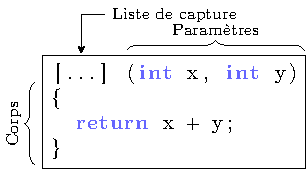
\includegraphics[height=3.5cm]{pics/lambda.pdf}}
%\end{center}
\end{frame}

\begin{frame}
\frametitle{Syntaxe}
\begin{center}
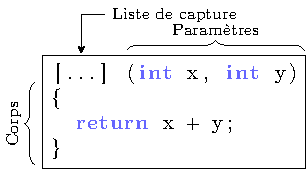
\includegraphics[height=3.5cm]{pics/lambda.pdf}
\end{center}
\begin{itemize}
\item Les paramètres et le corps du fonction sont spécifiés comme ceux d'une fonction «~habituelle~»
\item La liste de capture possède une syntaxe particulière, mais peut être vide
\end{itemize}
\end{frame}

\begin{frame}[containsverbatim]
\frametitle{Exemple}
\begin{itemize}
\item Fichier \texttt{lambda.cpp}
\item \texttt{std::for\_each} (\texttt{algorithm.h}) est une fonction appliquant une fonction donnée à tous les éléments d'un conteneur itérable
\end{itemize}
\begin{lstlisting}
int main()
{
	vector<int> v = {1, 2, 3, 4, 5};
	for_each(v.begin(), v.end(), [](int& i) { i++; });
	for_each(v.begin(), v.end(), [](int i) { cout << i << endl; });
}
\end{lstlisting}
\begin{itemize}
\item C'est « court »
\end{itemize}
\begin{alertblock}{Remarque}
	\begin{itemize}
	\item Avoir un code lisible est primordial
	\item Lambda courtes
	\end{itemize}
\end{alertblock}
\end{frame}

\begin{frame}
\frametitle{Déduction du type de retour}
\begin{itemize}
\onslide<1-> \item Dans l'exemple précédent, on n'a pas dû préciser le type de retour
\onslide<2-> \item Il est « déduit » par le compilateur
\onslide<3-> \item Si ce n'est pas possible (si \lstinline|auto| ne le permet pas), il faut le préciser
\end{itemize}
\begin{center}
\visible<4-|handout:1>{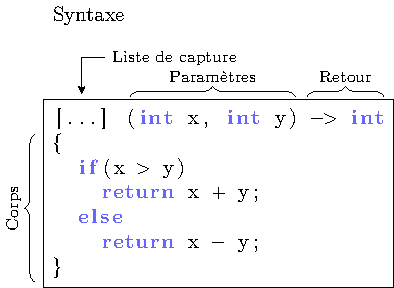
\includegraphics[height=4.5cm]{pics/lambda-ret.pdf}}
\end{center}
\end{frame}

\begin{frame}
\frametitle{Liste de capture}
\begin{itemize}[<+->]
\item Par défaut, rien en dehors des paramètres de la lambda ne peut être utilisé dans son corps
\item La liste de capture permet d'inclure des éléments « extérieurs »
\end{itemize}
\begin{exampleblock}<+->{Syntaxe}
	\begin{itemize}[<+->]
	\item \lstinline|[x]| : la variable \texttt{x} est passée par valeur
	\item \lstinline|[&x]| : la variable \texttt{x} est passée par référence
	\item \lstinline|[=]| : toutes les variables du bloc de déclaration sont passées par valeur
	\item \lstinline|[&]| : toutes les variables du bloc de déclaration sont passées par référence
	\end{itemize}
\end{exampleblock}
\begin{itemize}[<+->]
\item Possibilité de combinaison
	\begin{itemize}
	\item Par exemple : \lstinline|[x, &y]|
	\end{itemize}
\end{itemize}
\end{frame}

\begin{frame}[containsverbatim]
\frametitle{Exemple}
\begin{itemize}
\item Fichier \texttt{lambda-ret.cpp}
\end{itemize}
\begin{lstlisting}
struct A { int i; };

int main()
{
	A a; a.i = 1; 
	A b; b.i = 2;
	
	auto f = [&a, b] (int i) //generic lambda
		{
			int k = a.i + b.i + i;
			a.i += 3;
			//b.i += 3; //error, b is read-only

			return k;
		};

	cout << f(4) << endl;
	cout << a.i << " " << b.i << endl;
}
\end{lstlisting}
\end{frame}

\begin{frame}[containsverbatim]
\frametitle{Initialisation dans la liste de capture}
\begin{itemize}
\item En \cpp14, un élément de la liste de capture peut être initialisé
\end{itemize}
\begin{lstlisting}
int main()
{
	int x = 4;
	auto f = [&r = x, x = x + 1]()->int
	    {//r is a x-reference, x is incremented
	        r += 2;
	        return x + 2;
	    };//();

	int k = f(); //comment that and uncomment stuff before

	cout << x << endl; //6
	cout << k << endl; //7
}
\end{lstlisting}
\begin{alertblock}{Rappel}
	\begin{itemize}
	\item Avoir un code lisible est primordial
	\end{itemize}
\end{alertblock}
\end{frame}

\section{Constantes et inline}

\begin{frame}
\frametitle{CV-Qualifiers}
\begin{itemize}[<+->]
\item Pour chaque type, incluant les types incomplets, il existe trois autres « sous-types »
	\begin{enumerate}
	\item \lstinline|const| : type constant, accédé en lecture seule
	\item \lstinline|volatile| : type volatile, peut être modifié par un processus extérieur
	\item \lstinline|const volatile| : les deux en même temps
	\end{enumerate}
\item Motivation : optimisations compilatoires
	\begin{itemize}
	\item Un \lstinline|const| peut parfois être passé par référence
	\item Les instructions comprenant des volatiles ne peuvent être réordonnées
	\end{itemize}
\item Applications
	\begin{itemize}
	\item Optimisation de code
	\item Multithreading
	\end{itemize}
\end{itemize}
\end{frame}

\begin{frame}
\frametitle{Constantes}
\begin{itemize}[<+->]
\item Valeur ne changeant pas au cours de l'exécution du programme
\item Mot-clé \lstinline|const|
\item Réaffectation impossible
\item Utilisable sur des fonctions membres (\cpp)
	\begin{itemize}
	\item Ne modifie pas \lstinline|this|
	\item Cf. Ch. 4
	\end{itemize}
\item Objets (\cpp)
	\begin{itemize}
	\item Modification des attributs impossible
	\item Appel d'une fonction non constante impossible
	\end{itemize}
\end{itemize}
\end{frame}

\begin{frame}
\frametitle{Expressions \texttt{constexpr}}
\begin{itemize}[<+->]
\item Concept \cpp\ uniquement
	\begin{itemize}
	\item En \texttt{C}, il faut utiliser des macros
	\end{itemize}
\item Variable, fonction ou constructeur \emph{évaluable à la compilation}
\item Implique \lstinline|const| % et \lstinline|inline|
\item Utilisation du mot-clé \lstinline|constexpr|
\item Offre de grandes performances \emph{à l'exécution}
	\begin{itemize}
	\item Certains calculs sont effectués \emph{une fois} à la compilation
	\end{itemize}
\end{itemize}
\end{frame}

\begin{frame}
\frametitle{Variable \texttt{constexpr}}
\begin{exampleblock}<+->{Contraintes}
	\begin{enumerate}[<+->]
	\item Doit être un littéral
	\item Doit être immédiatement assigné ou construit
		\begin{itemize}
		\item Pas de déclaration sans assignation
		\item Les paramètres doivent être des littéraux, des constantes ou fonctions \lstinline|constexpr|
		\item Le constructeur doit être \lstinline|constexpr|
		\end{itemize}
	\end{enumerate}
\end{exampleblock}
\begin{itemize}[<+->]
\item Les contraintes ci-dessus offrent une possibilité d'évaluation et d'assignation de la variable à la compilation
\end{itemize}
\end{frame}

\begin{frame}
\frametitle{Fonction \texttt{constexpr}}
\begin{exampleblock}<+->{Contraintes}
	\begin{enumerate}[<+->]
	\item Ne peut pas être polymorphique
	\item Son type de retour doit être un littéral
	\item Les paramètres doivent être des littéraux, des constantes ou fonctions \lstinline|constexpr|
	\item Le corps ne peut pas contenir d'instruction non \lstinline|constexpr|
	\item Pas de \lstinline|try| / \lstinline|catch|
	\item Une seule instruction \lstinline|return| (pré \cpp 14)	
	\item Pas de définition de variable non littérale
	\item Etc.
	\end{enumerate}
\end{exampleblock}
\end{frame}

\begin{frame}[containsverbatim]
\frametitle{Exemple}
\begin{itemize}
\item Fichier \texttt{constexpr.cpp}
\item Ne prêtez pas attention à la \lstinline|struct| \texttt{constN}
	\begin{itemize}
	\item Affichage en compile-time
	\end{itemize}
\end{itemize}
\begin{lstlisting}
constexpr double PI = atan(1) * 4;

constexpr int factorial(int n)//c++11 : recursion, one return statement
{
    return n <= 1 ? 1 : n * factorial(n - 1);
}

constexpr long long int test(long long int n)//c++14
{
	int i = n;
	while(i >= 0)
		i--;
	return i;
}
\end{lstlisting}
\begin{itemize}
\item Un appel \texttt{test(9999999)} prend du temps à compiler
\end{itemize}
\end{frame}

\begin{frame}
\frametitle{Fonctions inline}
\begin{itemize}[<+->]
\item Fonction dont le corps est substitué à l'appel
\end{itemize}
\begin{exampleblock}<+->{Avantages}
	\begin{itemize}[<+->]
	\item Gain de temps (pas de \texttt{call})
	\end{itemize}
\end{exampleblock}
\begin{alertblock}<+->{Inconvénients}
	\begin{itemize}[<+->]
	\item Exécutable grossit (copier / coller)
	\end{itemize}
\end{alertblock}
\begin{itemize}[<+->]
\item Non contraignant : « demande courtoise »
\item Ces fonctions n'ont \emph{pas} d'adresse
\end{itemize}
\end{frame}

\begin{frame}
\frametitle{Contraintes}
\begin{itemize}[<+->]
\item Une fonction \lstinline|inline| est soit
	\begin{itemize}
	\item déclarée avec le mot-clé \lstinline|inline|
	\item implémentée dans le prototype de la classe (\cpp)
	\item une fonction \lstinline|constexpr| (\cpp)
	\end{itemize}
\end{itemize}
\begin{alertblock}<+->{Remarque}
	\begin{itemize}[<+->]
	\item Doit être déclarée et implémentée au sein du même fichier
	\item Ne peut pas être utilisée là où l'adresse d'une fonction est attendue
	\end{itemize}
\end{alertblock}
\end{frame}

\begin{frame}[containsverbatim]
\frametitle{Exemple}
\begin{itemize}
\item Fichier \texttt{inline.h}
\end{itemize}
\begin{lstlisting}
struct A
{
	void f() //inline
	{
		cout << "Brol::f" << endl;
	}
};

struct B
{
	inline void f();//inline
};

void B::f()
{
	cout << "Foo::f" << endl;//defined in same file
}

inline double sum(double a, double b) { return a + b; } //inline

struct C
{
	void f();//not inline
};
\end{lstlisting}
\end{frame}

\begin{frame}[containsverbatim]
\frametitle{Exemple}
\begin{itemize}
\item Fichiers \texttt{inline.cpp}, \texttt{inline-main.cpp}
\end{itemize}
\begin{lstlisting}
void C::f()
{
	cout << "C::f" << endl;
}
\end{lstlisting}
\begin{lstlisting}
int main()
{
	A a;
	a.f();

	B b;
	b.f();

	C c;
	c.f();
	
	cout << sum(2,3) << endl;
}
\end{lstlisting}
\end{frame}

\section{Les lvalue}

\begin{frame}
\frametitle{Intuition}
\begin{exampleblock}<+->{lvalue}
	\begin{itemize}[<+->]
	\item «~Valeur qui peut apparaître à gauche d'un opérateur d'affectation~»
	\end{itemize}
\end{exampleblock}
\begin{itemize}[<+->]
\item Définition insuffisante
\end{itemize}
\begin{alertblock}<+->{Remarque}
	\begin{itemize}[<+->]
	\item \lstinline|const int a = 2; //ok|
	\item \lstinline|a = 3; //ko|
	\end{itemize}
\end{alertblock}
\end{frame}

\begin{frame}
\frametitle{Notion de lvalue}
\begin{exampleblock}<+->{Intuition}
	\begin{itemize}[<+->]
	\item \lstinline|double x, y, a, b;|
	\item \lstinline|y = a*x + b; //ok|
	\item \lstinline|a*x + b = y; //ko|
	\item \lstinline|(x + 1) = 4; //ko|
	\end{itemize}
\end{exampleblock}
\begin{itemize}[<+->]
\item Le premier opérande \emph{doit} référencer un emplacement mémoire non temporaire
	\begin{itemize}
	\item Autres langages : variable, en \texttt{C} / \cpp, pas assez précis
%	\item Pas assez précis en \texttt{C} / \cpp
	\end{itemize}
\item Contrainte nécessaire à plusieurs endroits dans le langage % (\texttt{=}, \texttt{++}, références, etc.)
\item Propriété très importante pour les \emph{expressions}
%	\begin{itemize}
%	\item En dépit du nom
%	\end{itemize}
\item Ce qui n'est pas une \texttt{lvalue} est une \emph{rvalue} (immédiats, temporaires, anonymes, etc.)
\end{itemize}
\end{frame}

\begin{frame}
\frametitle{Conversions entre lvalues et rvalues}
\begin{itemize}[<+->]
\item Souvent, les opérateurs (et fonctions) requièrent des arguments rvalues
\end{itemize}
\begin{exampleblock}<+->{Exemple}
	\begin{itemize}
	\item \lstinline|int i = 1;|
	\item \lstinline|int j = 2;|
	\item \lstinline|int k = i + j;|
	\end{itemize}
\end{exampleblock}
\begin{enumerate}[<+->]
\item \texttt{i} et \texttt{j} sont des lvalue
\item \texttt{+} requiert des rvalue
\item \texttt{i} et \texttt{j} sont convertis en rvalue
\item Une rvalue est retournée
\end{enumerate}
\end{frame}

\begin{frame}
\frametitle{Règles de conversions}
\begin{exampleblock}<+->{Conversion lvalue vers rvalue}
	\begin{itemize}[<+->]
	\item Toutes les lvalues qui ne sont pas des tableaux, des fonctions et des types incomplets peuvent être convertis en rvalues
	\end{itemize}
\end{exampleblock}
\begin{alertblock}<+->{Conversion rvalue vers lvalue}
	\begin{itemize}[<+->]
	\item Impossible implicitement
	\item Le résultat d'un opérateur (rvalue) peut être explicitement affecté en une lvalue
	\end{itemize}
\end{alertblock}
\begin{itemize}[<+->]
\item On peut produire des lvalue à partir de rvalue explicitement
	\begin{itemize}
	\item Le déférencement prend une rvalue et produit une lvalue
	\item L'opérateur \texttt{\&} prend une lvalue et produit une rvalue
	\end{itemize}
\end{itemize}
\end{frame}

\begin{frame}[containsverbatim]
\frametitle{Exemple}
\begin{itemize}
\item Fichier \texttt{rvalue-conv.cpp}
\end{itemize}
\begin{lstlisting}
int main()
{
	int a[] = {1, 2};
	int* pt = &a[0];
	*(pt + 1) = 10;   //OK : p + 1 is an rvalue, but *(p + 1) is an lvalue

	//taking adress
	int i = 10;
	//int* pti = &(i + 1);   // KO : lvalue required
	int* pti = &i;           // OK: i is an lvalue
	//&i = 20;               // KO : lvalue required

	//reference making
	//std::string& sref = std::string(); //KO : non const-ref init from rvalue
}
\end{lstlisting}
\end{frame}

\begin{frame}[containsverbatim]
\frametitle{Références de \texttt{lvalue}}
\begin{itemize}
\item Fichier \texttt{lvalue-ref.cpp}
\end{itemize}
\begin{lstlisting}
int n = 5;
int& truc = n;

int& brol() { return n; }

int main() {
	cout << brol() << endl;
	brol() = 10;
	cout << brol() << endl;

	truc = 15;
	cout << brol() << endl;

	//int & i = 2;
}
\end{lstlisting}
\begin{itemize}
\item \texttt{n} est une \texttt{lvalue}, \texttt{brol()} aussi
\item Les références de \texttt{lvalue} sont des \texttt{lvalue}
	\begin{itemize}
	\item Utile pour l'opérateur \texttt{[]}
	\item \texttt{v[10] = 42;}
	\end{itemize}
\end{itemize}
\end{frame}

\begin{frame}[containsverbatim]
\frametitle{La motivation des contraintes}
\begin{itemize}
\item On ne veut pas pouvoir réaffecter un temporaire / immédiat
\end{itemize}
\begin{lstlisting}
int a = 42;
int b = 43;

 // a and b are both lvalues:
a = b; // ok
b = a; // ok
a = a * b; // ok

// a * b is an rvalue:
int c = a * b; // ok, rvalue on right hand side of assignment
a * b = 42; // error, rvalue on left hand side of assignment

//2 is a rvalue
int d = 2;
int & d = 2; //error
const int& e = 2; //ok : you are allowed to bind a const lvalue to a rvalue
\end{lstlisting}
\begin{itemize}
\item Il existe néanmoins des références de rvalue (Cf. Ch. 9)
\item Le fait qu'une expression soit une rvalue ou une lvalue est appelé la \emph{value category}
\end{itemize}
\end{frame}

\section{Règles d'appel}

\begin{frame}
\frametitle{Surdéfinition}
\begin{itemize}[<+->]
\item On parle de surdéfinition (overloading) quand un même symbole possède plusieurs significations
\item Le choix du symbole dépend du contexte
\end{itemize}
\begin{exampleblock}<+->{Exemple : \texttt{a + b}}
	\begin{itemize}[<+->]
	\item Addition entière
	\item Addition flottante
	\end{itemize}
\end{exampleblock}
\begin{itemize}[<+->]
\item En \cpp, on peut surdéfinir des fonctions
	\begin{itemize}
%	\item Ce qui inclut la plupart des opérateurs
	\item Des règles d'appel sont mises en œuvre pour le choix de la fonction à appeler en cas «~d'ambiguïté~»
	\end{itemize}
\item En \texttt{C}, seul ne nom de la fonction à appeler intervient dans la recherche
	\begin{itemize}
	\item Le seul overload existant est celui avec les opérateurs arithmétiques et le types de base
	\end{itemize}
\end{itemize}
\end{frame}

\begin{frame}
\frametitle{Étapes dans l'appel d'une fonction en \cpp}
\begin{enumerate}[<+->]
\item Name lookup
	\begin{itemize}
	\item On recherche la définition d'un symbole
	\item Pour des fonctions, cette recherche dépend du type des arguments
	\item Pour des templates, il faut déduire le type des arguments (cf. Ch. 13)
	\end{itemize}
\item Si ces étapes produisent plus d'une correspondance (surdéfinition), il faut résoudre l'ambiguïté
	\begin{itemize}
	\item Overload resolution
	\item En pratique, on cherche la «~meilleure correspondance~»
	\item Les conversions ont un «~score~» (rank)
		\begin{itemize}
		\item Les conversions de meilleur score sont privilégiées
		\item Si on a le choix entre deux conversions de même score : erreur
		\end{itemize}
	\end{itemize}
\item Si elle ne peut pas être résolue : erreur
	\begin{itemize}
	\item Aucune définition meilleure qu'une autre
	\end{itemize}
\end{enumerate}
\end{frame}

\begin{frame}
\frametitle{Choix de fonction à appeler}
\begin{itemize}[<+->]
\item Idée : le compilateur cherche « la meilleure » correspondance possible
\end{itemize}
\begin{alertblock}<+->{Règles d'appel}
	\begin{enumerate}[<+->]
	\item Correspondance exacte
		\begin{itemize}
		\item Tous les types sont distingués
		\item \lstinline|const| intervient uniquement dans le cas de pointeurs et références
		\end{itemize}
	\item Correspondance de type «~promotion~»
		\begin{itemize}
		\item Promotion entière, promotion flottante
		\end{itemize}
	\item Autres conversions
		\begin{itemize}
		\item Conversion entière, conversion flottante, conversion \lstinline|void*|, conversion définie par l'utilisateur (\cpp), etc.
		\end{itemize}
	\end{enumerate}
\end{alertblock}
%\begin{itemize}[<+->]
%\item En pratique, les conversions ont un «~score~» (rank)
%	\begin{itemize}
%	\item Les conversions de meilleur score sont privilégiées
%	\item Si on a le choix entre deux conversions de même score : erreur
%	\end{itemize}
%\end{itemize}
\end{frame}

\begin{frame}[containsverbatim]
\frametitle{Exemple}
\begin{itemize}
%\item Cas des références de rvalue : on privilégie un prototype explicite
\item Fichier \texttt{surdef.cpp}
\end{itemize}
\begin{lstlisting}
int f(int i) {
	cout << "Integer " << i << endl; 
	return 0;
}

//double f(int i) {} //return type matters not
//int f(const int i) {} //cv-qualifier lost

int f(double d) {
	cout << "Double " << d << endl;
	return 0;
}

int f(int i, int j) {
	cout << "Integers " << i << " and " << j << endl;
}

int main() {
	int k = 1;
	f(k);
	double d = 2.1;
	f(d);
	f(k,d);
}
\end{lstlisting}
\begin{itemize}
\item Impossible en \texttt{C} (fichier \texttt{surdef.c})
\end{itemize}
\end{frame}

\begin{frame}
\frametitle{rvalue et cv-qualifiers}
\begin{exampleblock}<+->{Conversions de rvalue cv-qualifiée}
	\begin{itemize}[<+->]
	\item Une lvalue de type \texttt{T} qui n'est ni une fonction ni un tableau peut être convertie en rvalue.
		\begin{enumerate}
		\item Si ce n'est pas une classe, le type de la rvalue est la version cv non qualifiée de \texttt{T}
		\item Sinon, le type de la rvalue est \texttt{T}
		\end{enumerate}
	\end{itemize}
\end{exampleblock}
\begin{alertblock}<+->{Conséquence}
	\begin{itemize}[<+->]
	\item Les cv-qualifiers sont perdus sur les arguments explicites
	\item Pas sur \lstinline|this|
	\end{itemize}
\end{alertblock}
\end{frame}

\begin{frame}[containsverbatim]
\frametitle{Exemple}
\begin{itemize}
\item Fichier \texttt{const-call.cpp}
\item Ne vous souciez pas de \lstinline|struct|
	\begin{itemize}
	\item « Comme une classe » (cf. Ch. 4)
	\end{itemize}
\end{itemize}
\begin{lstlisting}
struct A
{
    void brol() const { cout << "A::brol() const" << endl; }
    void brol() { cout << "A::brol()" << endl; }

    void brol2(A) { cout << "A::brol2(A)" << endl; }
    
    //ERROR : cv-qualifier lost
    //void brol2(const A) { cout << "A::brol2(const A)" << endl; } 
};

int main()
{
    A a = A();//creates an A (rvalue to lvalue conv)
    const A ca = A();//creates an A (rvalue to lvalue conv)

    a.brol();  //brol
    ca.brol(); //brol const

    a.brol2(a);
    a.brol2(ca);
}
\end{lstlisting}
\end{frame}

\begin{frame}
\frametitle{Contraintes références}
\begin{itemize}[<+->]
\item Une fonction \lstinline|void f(int&);| est appelée avec une référence
\item \emph{Doit} être une lvalue
\end{itemize}
\begin{alertblock}<+->{Conséquences}
	\begin{itemize}[<+->]
	\item Pas d'immédiat
	\item Pas d'expression
	\item Pas de conversion ou tronquage
	\end{itemize}
\end{alertblock}
\begin{itemize}[<+->]
\item Idée : sinon, on pourrait changer la valeur d'un temporaire, écrire \texttt{a*x+b = y;}, etc.
\item Différent avec \lstinline|const|
\end{itemize}
\end{frame}

\begin{frame}[containsverbatim]
\frametitle{Exemple}
\begin{itemize}
\item Fichier \texttt{ref-cstr.cpp}
\end{itemize}
\begin{lstlisting}
void f(int&){}

int main()
{
	const int n = 15;
	int q;
	f(q);
	//f(2*q+3);//not a lvalue
	//f(3);
	//f(n);//wrong cv-qualifier

	float x;
	//f(x);//no truncation

	short k;
	//f(k);//no conversion
}
\end{lstlisting}
\end{frame}

\begin{frame}
\frametitle{Exceptions}
\begin{itemize}[<+->]
\item Le prototype d'une fonction peut prendre par référence des paramètres constants
\end{itemize}
\begin{exampleblock}<+->{Exemple}
	\begin{itemize}[<+->]
	\item \lstinline|void f(const int& n);|
	\end{itemize}
\end{exampleblock}
\begin{itemize}[<+->]
\item Ici, il est prévu que les paramètres soient constants, et donc non modifiables
\item Permet un appel de \texttt{f} sur \emph{toute} expression entière
	\begin{itemize}
	\item \texttt{f(2)}, \texttt{f(3 * n)}, etc.
	\item Conversions placées dans des variables temporaires transmises par référence
	\item Risque de modification de temporaire supprimé
	\end{itemize}
\end{itemize}
\end{frame}

\begin{frame}[containsverbatim]
\frametitle{Exemple}
\begin{itemize}
\item Fichier \texttt{surdef-ref.cpp}
\end{itemize}
\begin{lstlisting}
void f(int & i)
{
	cout << "Ref " << i << endl;
}

void f(const int & i)
{
	cout << "Ref cst " << i << endl;
}

int main()
{
	int n = 3;
	const int m = 5;
	f(n);
	f(3);
	f(int{4});
	f(4 * n);
	f(4 * m);
	f(m);
}
\end{lstlisting}
\end{frame}

\begin{frame}[containsverbatim]
\frametitle{Le cas des pointeurs}
\begin{itemize}
\item Fichier \texttt{surdef-ptr.cpp}
\end{itemize}
\begin{lstlisting}
//void brol(char*) { cout << "Brol char" << endl; }
void brol(double*) { cout << "Brol double" << endl; }
void brol(void*) { cout << "Brol void" << endl; }
void brol(int*) { cout << "Brol int" << endl; }
//void brol(int* const) { cout << "int const" << endl; } //try to uncomment that
void brol(const int*) { cout << "Const int" << endl; }

int main()
{
	char * ptc;
	double * ptd;
	void* ptv;
	
	brol(ptc);// char, try when remove brol(char*) -> void
	brol(ptd);// double		
	brol(ptv);//remove brol(void*) for this call : ERROR (no conv)

	int n = 3;
	const int p = 5;

	brol(&n);
	brol(&p);		
}
\end{lstlisting}
\end{frame}
\end{document}
